\documentclass[aspectratio=169]{beamer}
\usepackage[utf8]{inputenc}

\usepackage{xcolor}
 \definecolor{redp}{rgb}{0.78, 0.03, 0.08}
\definecolor{greenp}{rgb}{0.0, 0.51, 0.5}
\definecolor{yellowp}{rgb}{0.59, 0.44, 0.09}

\newcommand{\enb}[1]{\textcolor{poliblue1}{\textbf{#1}}}
\newcommand{\eno}[1]{\textcolor{orange}{\textbf{#1}}}
\definecolor{softblue}{cmyk}{.2, .1, .1, .2}
\newcommand{\soft}[1]{\textcolor{softblue}{#1}}

\DeclareMathOperator*{\EV}{\mathbb{E}}
\newcommand{\EVV}[2][\ppvect \in \ppspace]{\EV_{#1}\left[{#2}\right]}
\newcommand{\norm}[2][\infty]{\left\|#2\right\|_{#1}}

\title{Stochastic Variance-Reduced Policy Gradient}
\date[ICML 2018]{\small{35\textsuperscript{th} International Conference on Machine Learning, Stockholm, Sweden}}
\author[Papini et al.]{\textbf{Matteo Papini} \\
						\small{Damiano Binaghi \quad Giuseppe Canonaco \\
								Matteo Pirotta \quad Marcello Restelli}}

\usetheme{polimithx}
\usetikzlibrary{calc}

%%%%%%%%%%%%%%%%%%%%%%%%%% BIBLIOGRAPHY
\usepackage{natbib}
\bibliographystyle{apalike}
% make bibliography entries smaller
\renewcommand\bibfont{\scriptsize}
% If you have more than one page of references, you want to tell beamer
% to put the continuation section label from the second slide onwards
\setbeamertemplate{frametitle continuation}[from second]

%CUSTOM COMMANDS
\newcommand{\vtheta}{\boldsymbol{\theta}}

\begin{document}

\setbeamertemplate{caption}{\raggedright\insertcaption\par}

\begin{frame}
\titlepage
\end{frame}

\begin{frame} 
\frametitle{Outline} 
\begin{center}
	\Large{\enb{S}\soft{tochastic}
		\enb{V}\soft{ariance-}}\enb{R}\soft{educed}
	\soft{(}\enb{P}\soft{olicy}\soft{)}
	\enb{G}\soft{radient}
\end{center}


\begin{itemize}
	\item \enb{SVRG} for Reinforcement Learning
		\begin{itemize}
		\item Motivation
		\item Challenges
	\end{itemize}
	\item \enb{SVRPG}
	\begin{itemize}
		\item Convergence Properties
		\item Heuristics
		\item Experiments
	\end{itemize}
\end{itemize}

\end{frame}

\begin{frame} 
\frametitle{Policy Gradient} 
An effective \enb{Reinforcement Learning (RL)} solution to \enb{continuous} control problems:

\begin{minipage}[t]{.4\paperwidth}
\begin{figure}
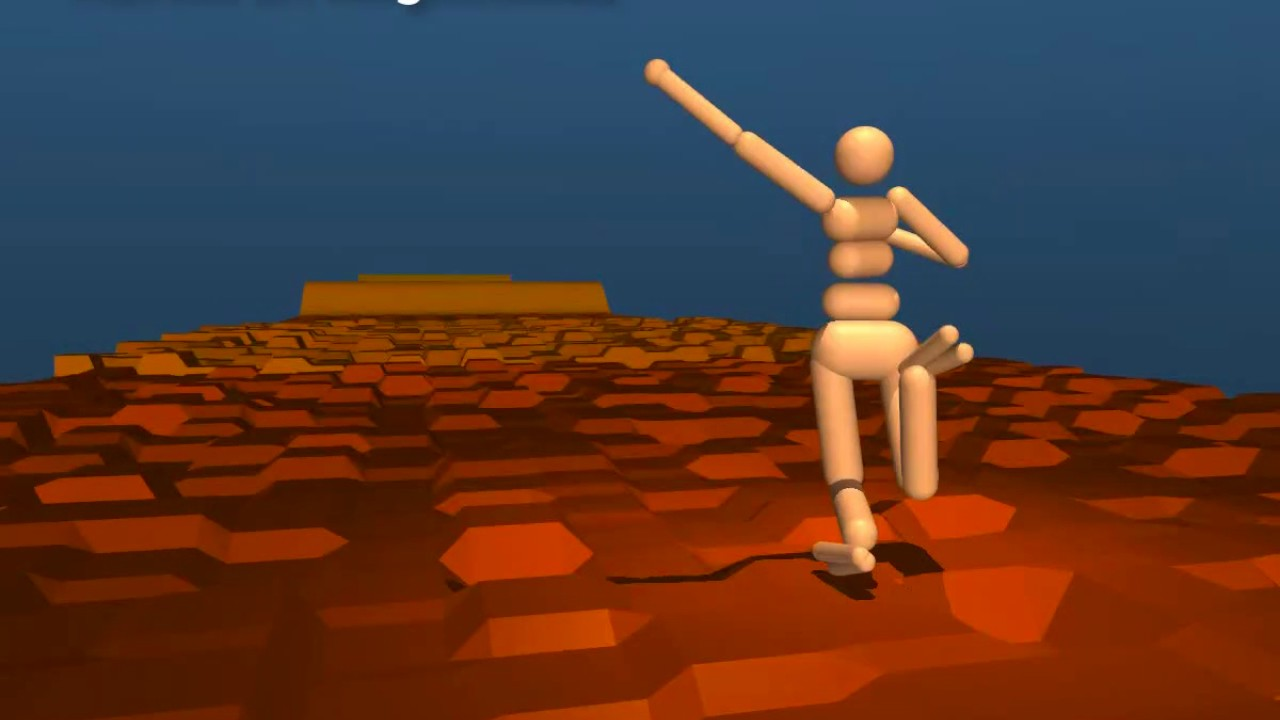
\includegraphics[width=\textwidth]{images/parkour.jpg}
\caption{Robotics~\citep{heess2017emergence}}
\end{figure}
\end{minipage}
\hfill%
\begin{minipage}[t]{.4\paperwidth}
\begin{figure}
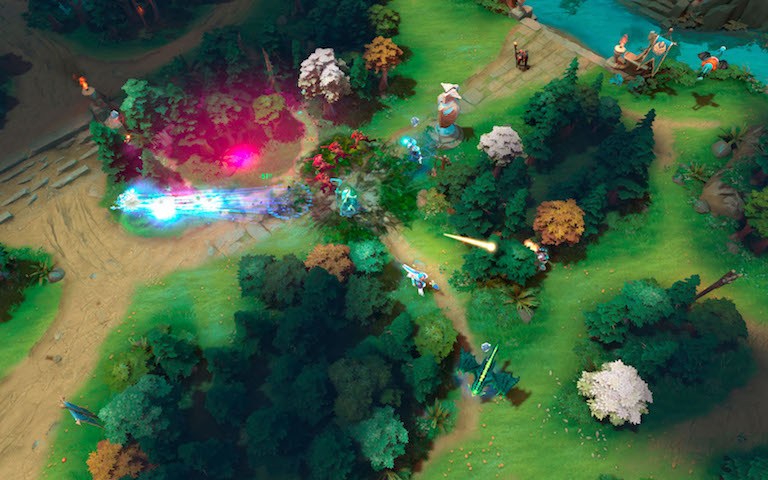
\includegraphics[width=\textwidth, height=3.6cm]{images/dota.jpg}
\caption{Video games~\citep{openaifive}}
\end{figure}	
\end{minipage}

\vspace*{.5cm}

\large{Mostly based on \enb{Stochastic Gradient Ascent}~\citep{robbins1951stochastic}}

\end{frame}

\begin{frame} 
\frametitle{Full vs Stochastic Gradient} 
\textit{Plot: visualizing rates of convergence}

\Large{\enb{Can we do something better?}}

\end{frame}

\begin{frame} 
\frametitle{SVRG} 
\framesubtitle{Stochastic Variance-Reduced Gradient}
A solution from \enb{finite-sum optimization}:

\begin{align*}
	&\Large{
	\textcolor{poliblue3}{\underbrace{\blacktriangledown J(\vtheta)}_{\text{SVRG estimator}}}
	= \textcolor{greenp}{\underbrace{\nabla J(\widetilde{\vtheta}) }_{\text{FG in snapshot parameter}}}
	+ \textcolor{redp}{\underbrace{\nabla J(\vtheta)\rvert_{\tau_i}}_{\text{SG in current parameter}}}
	- \textcolor{yellowp}{\underbrace{\nabla J(\widetilde{\vtheta})\rvert_{\tau_i}}_{\text{Correction term}}}}
\end{align*}

\begin{itemize}
	\item Unbiased
	\item Linear convergence
	\item More data-efficient than FG
	\item Easily applicable to \enb{Supervised Learning (SL)}
\end{itemize}
\end{frame}

\begin{frame} 
\frametitle{SVRG for Reinforcement Learning}
\framesubtitle{Stochastic Variance-Reduced Gradient} 
Not trivial! There are three \eno{challenges}:

\vspace*{.5cm}
\begin{enumerate}
	\item \eno{Non-concavity} of $J(\vtheta)$
		\citep{allen2016variance,reddi2016stochastic}
	\item \eno{Infinite dataset}: we would need \textit{infinite samples} to compute FG~\citep{harikandeh2015stopwasting,bietti2017stochastic}
	\item \eno{Non-stationarity}: $\tau\sim p_{\textcolor{orange}\vtheta}$ (new!)
\end{enumerate}


RL so far: \textit{policy evaluation}~\citep{du2017svrgpe} and \textit{off-policy control}~\citep{xu2017svrgtrpo}

\vspace*{.5cm}

Our work: \enb{on-policy control}

\end{frame}

\begin{frame} 
\frametitle{SVRPG} 
\framesubtitle{Stochastic Variance-Reduced \textbf{Policy} Gradient}



\begin{equation*}
\LARGE{
	\textcolor{poliblue3}{\underbrace{\blacktriangledown J(\vtheta)}_{\text{SVRPG estimator}}}
	= \textcolor{greenp}{\underbrace{\widehat{\nabla}_N J(\widetilde{\vtheta}) }_{\text{\shortstack{Large N\\to approximate FG}}}}
	+ \textcolor{redp}{\underbrace{\widehat{\nabla}_B J(\vtheta)}_{B << N}}
	- \textcolor{yellowp}{\underbrace{\omega(\vtheta,\widetilde{\vtheta})\widehat{\nabla}_B J(\widetilde{\vtheta})}_{\text{\shortstack{Importance weighting\\for non-stationarity}}}}}
\end{equation*}

\begin{itemize}
	\item Unbiased
	\item More data-efficient than FG
\end{itemize}

\end{frame}

\begin{frame} 
\frametitle{Convergence Properties} 
Convergence to \eno{local} optimum:

\Large{
\begin{equation*}
	\EVV[]
	{\norm[]{\nabla J(\vtheta)}^2} 
	\leq
	\frac{J(\vtheta^*)-J(\vtheta_0)}{\psi T} +
	\textcolor{orange}{\underbrace{\frac{\zeta}{N}}_{\text{Infinite dataset}}}
	+\textcolor{orange}{\underbrace{\frac{\xi}{B}}_{\text{Nonstationarity}}}
\end{equation*}
}

\begin{itemize}
	\item Linear convergence $+$ error~\citep [similar to][]{harikandeh2015stopwasting}
\end{itemize}

\end{frame}

\begin{frame} 
\frametitle{Heuristics} 
Meta-parameter selection

\begin{itemize}
	\item \enb{Adaptive step size}: two ADAM annealing schedules
	 \begin{equation*}
	 	\underbrace{\alpha_{FG}}_{\text{used at the snapshot}} \qquad \underbrace{\alpha_{SG}}_{\text{used inside epoch}}
	 \end{equation*}
	\item \enb{Adaptive epoch size}: take new snapshot when the effective step size becomes too small
	\begin{equation*}
		\frac{\alpha_{SG}}{B} < \frac{\alpha_{FG}}{N} \implies \textbf{snapshot}
	\end{equation*}
\end{itemize}

\end{frame}

\begin{frame} 
\frametitle{Results} 

%\begin{tikzpicture}

\begin{minipage}[t]{.28\paperwidth}
\begin{center}
	\textbf{Cart-Pole}
\end{center}
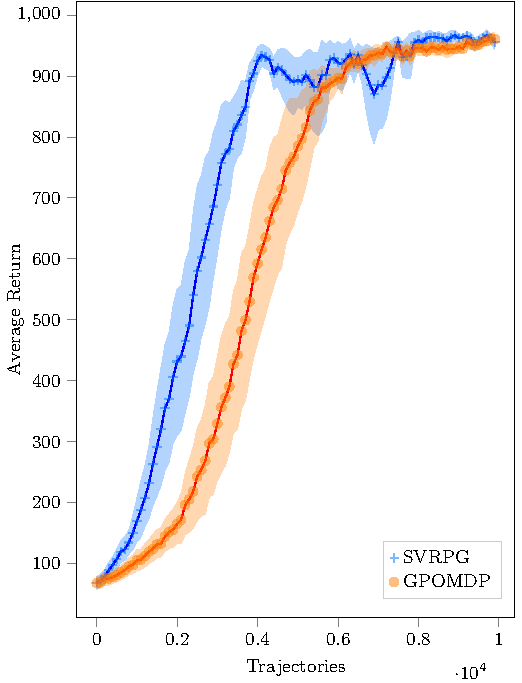
\includegraphics[width=\textwidth]{images/cartpole.pdf}
\end{minipage}
%
\begin{minipage}[t]{.28\paperwidth}
\begin{center}
	\textbf{Swimmer}
\end{center}
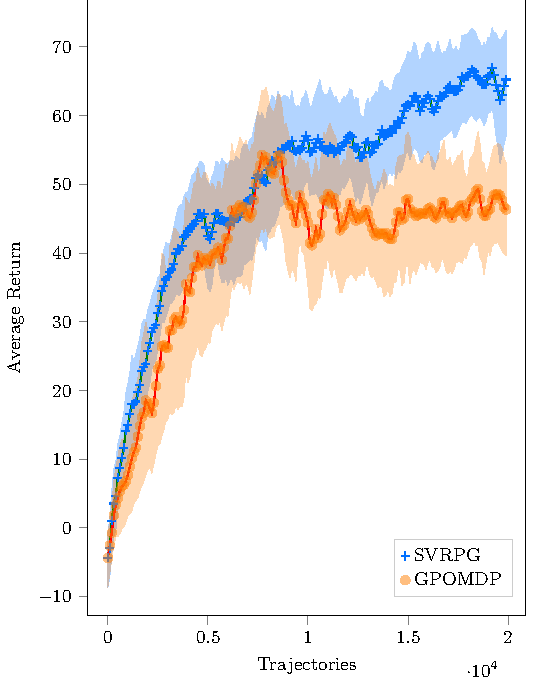
\includegraphics[width=\textwidth]{images/swimmer.pdf}
\end{minipage}
%
\begin{minipage}[t]{.28\paperwidth}
\begin{center}
	\textbf{Half-Cheetah}
\end{center}
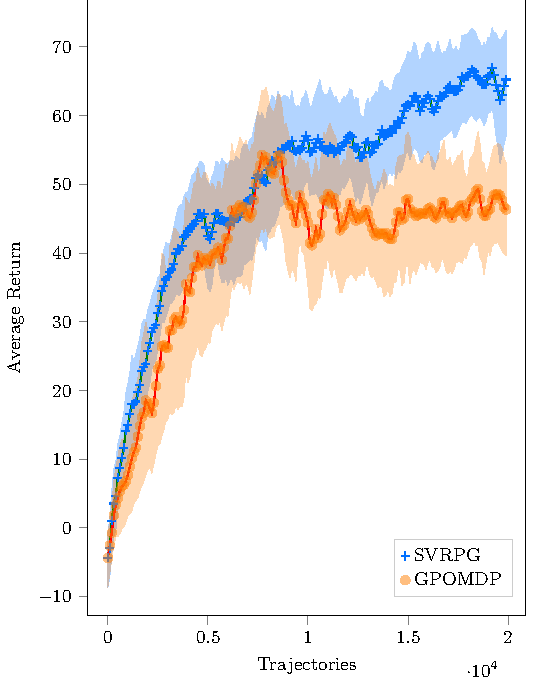
\includegraphics[width=\textwidth]{images/swimmer.pdf}
\end{minipage}

%\node[inner sep=0pt] (picture1) {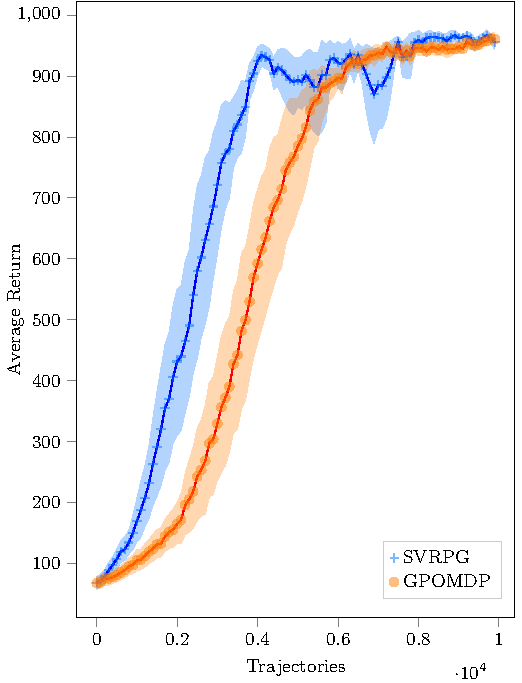
\includegraphics[width=.32\textwidth]{images/cartpole.pdf}};
%\node[above left] at ($(picture1.north) + (1.3cm,0)$) {\textbf{Cart-Pole}};
%\end{tikzpicture}
%%
%\begin{tikzpicture}
%\node[inner sep=0pt] (picture2) {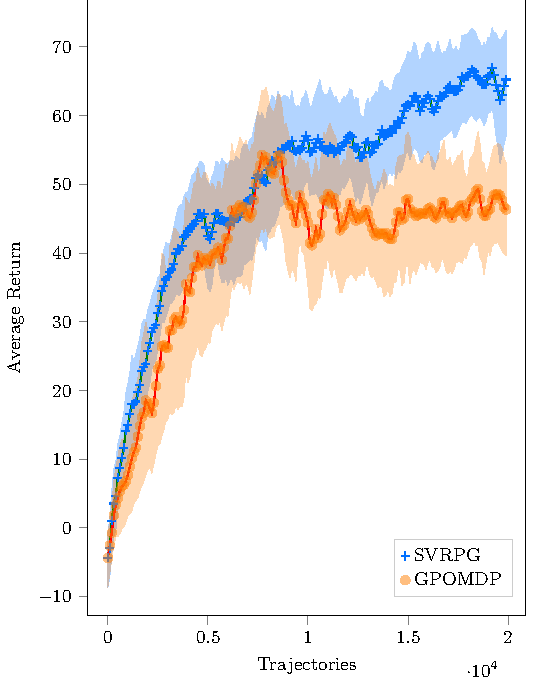
\includegraphics[width=0.32\textwidth]{images/swimmer.pdf}};
%\node[above left] at ($(picture1.north) + (1.3cm,0)$) {\textbf{Swimmer}};
%\end{tikzpicture}
%%
%\begin{tikzpicture}
%\node[inner sep=0pt] (picture3) {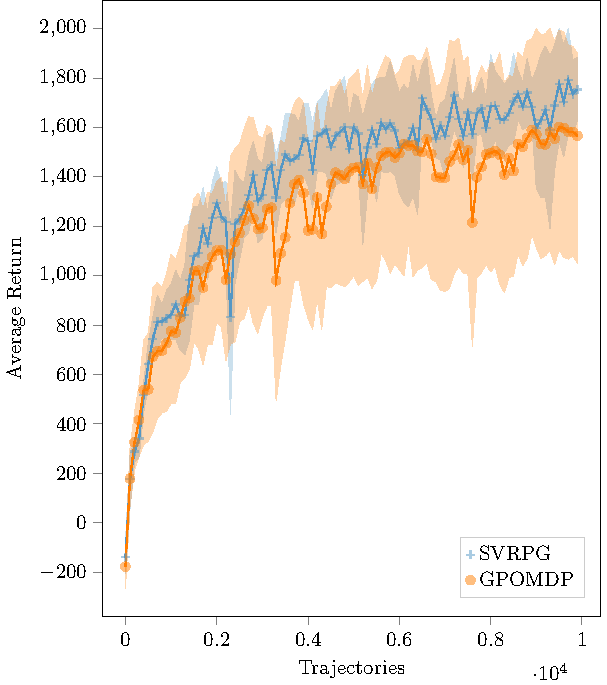
\includegraphics[width=0.32\textwidth]{images/cheetah.pdf}};
%\node[above left] at ($(picture1.north) + (1.3cm,0)$) {\textbf{Half-Cheetah}};
%\end{tikzpicture}%

\end{frame}

\begin{frame} 
\frametitle{Conclusions} 

\begin{itemize}
	\item Efficient policy optimization is challenging
	\item \enb{SVRPG}: on-policy control based on SVRG
	\item Meta-parameters still crucial to tame different sources of variance
	\item Future work: adaptive batch size, natural gradient, actor-critic
\end{itemize}

\end{frame}


\begin{frame} 
\frametitle{Thank You} 
\begin{center}
	\Large{\enb{Thank you for your attention}}
\end{center}

\begin{minipage}[]{.6\paperwidth}
\begin{itemize}
	\item Poster: today 06:15 -- 09:00 PM @ \enb{Hall B \#65} 
	\item Contact: \texttt{matteo.papini@polimi.it}
	\item Online resources: \texttt{t3p.github.io}
	\end{itemize}
\end{minipage}
\hfill%
\begin{minipage}[]{.2\paperwidth}

\includegraphics[width=.2\paperwidth]{../qrcode.pdf}
\end{minipage}

\end{frame}


%%%%%%%%%%%%%%%%%%%%%%%%%%%%%%%%%%%%%%%%%%%%%%%%%%%%%%%%%%%%%%%%%%%%%%%%%%%%%%%%%%%%%%%%%
\begin{frame}[allowframebreaks,fragile]
\frametitle{References}
\bibliography{talk.bib}
\end{frame}
%%%%%%%%%%%%%%%%%%%%%%%%%%%%%%%%%%%%%%%%%%%%%%%%%%%%%%%%%%%%%%%%%%%%%%%%%%%%%%%%%%%%%%%%%

%%Backup Slides
\begin{frame} 
\frametitle{Adaptive Step Size} 


\end{frame}

\begin{frame} 
\frametitle{Adaptive Epoch Size} 


\end{frame}

\begin{frame} 
\frametitle{Normalized Importance Weights} 


\end{frame}

\begin{frame} 
\frametitle{Actor-Critic SVRPG} 


\end{frame}

\begin{frame} 
\frametitle{The Full Comparison} 


\end{frame}

\end{document}